\chapter{定量脑电中电势影响因素:参考模态与电极配置}
\section{引言}
自从1929年人类脑电的发现,头表脑电因为其敏感性、无创性、高时间分辨率等优点已成为大脑研究不可或缺的工具。认知科学家、临床医生、工程师们正在使用脑电分别讲述在认知心理学,神经病精神疾病学以及虚拟现实脑机接口等领域成功应用脑电的故事。脑电的成功应用通常依赖于信号处理方法,包括对时域信号的时频分析\cite{konig2001topographic},头皮表面的地形图分析\cite{lehmann1971multichannel},以及大脑源空间的层析成像分析\cite{pascual1999review}。这些分析要求对源模型\cite{scherg1990fundamentals}、头模型、容积传导模型的准确估计或模拟,但最重要的是更加接近准确的脑电电势记录。

为了获得准确的头表记录,我们不仅需要控制各种各样的环境噪声也需要减少非中立零参考的失真效应。原则上,脑电电势是活跃电极与参考电极之间的电势差\cite{nunez1997eeg}。在过去的几十年间,人们一直在追求一种接近的零参考电极,以至于活跃电极能够局部记录到时变电势。然而,在身体表面找到一种不活动或者中立的位点是不可能的。参考的选择还没有得到较好地解决,形成了不一致的用法和无休止的讨论,这就是所谓的“参考电极问题”。 目前,多种多样的参考模态已经提出,包括在线记录参考(常用的各种单点参考),和几种离线重参考如连接耳参考(LM)\cite{garneski1958equalizing},平均参考(AR)\cite{offner1950eeg},和参考电极标准化技术(REST)\cite{yao2001method}。以前的研究表明参考的选择对脑电波形和功率谱\cite{rellecke2013emotion,chella2017non}有重大影响,然后参考的效果受到各种因素特别是电极数目的影响\cite{liu2015estimating,chella2016impact,lei2017understanding}。

在当前的实际应用中,电极数目参差不齐变动范围很大:如临床中常用10导联或者16导联,认知神经科学研究中常采用64-256导联的高密度阵列,甚至在一些研究中用到多于300导联的超高维阵列\cite{jurcak200710,oostenveld2001five}。然而,以前对于电极导联数对于重参考效果的的研究局限于21-256导联。现在,我们绝地有必要进行覆盖从10导联到300导联以上的对电极数目进行综合的评价研究。此外,随着电极数目增多,这些电极是怎样分布在头表的呢? 典型地具有21电极数目的国际10-20标准放置系统是标准化电极分布的第一份建议\cite{676199734}。 然后,10-10和10-5系统是10-20系统的衍生,只是采用了更多的电极并加以命名以满足先进的源成像技术的需要\cite{10016997968, chatrian1985ten}。 也就是说,这些系统在原来10-20系统的电极基础上按照相对头表面基于的位置准则定义了更多的电极位置。在本研究中,这一系列系统被成为“10-x”系统。相反,另外一种电极分布有Electrical Geodesics, Inc. (USA) 提出,致力于进行高密度脑电神经成像\cite{676199764} 思路是按照测地传感网络(GSN)放置更多的电极,好似是在球面上剖分多边形并指定多边形的中心作为电极位置\cite{tucker1993spatial}。 这里,这种电极分布系统被成为“GSN”分布。这两种电极分布的主要差别在于电极是否也覆盖到面颊和颈部。 在不同的电极分布下,重参考技术矫正电位失真的效果是怎样呢?这个问题过去一直被不自觉地忽视。

本章中我们同时研究了参考模态和电机配置(包括电极导联数目和电极分布)两个主要因素。 最初,我们用各种电极配置通过正演计算仿真生成具有无穷远参考的标准脑电电位。 接下来,标准的无穷远参考下的脑电电位被变换为单点参考记录以及三种典型的重参考(LM,AR 和 REST)。 随后, 无穷远参考下的正演出的电位与其他参考下的相对误差计算出来,显然,这种误差取决于 电极数目和电极分布等因素。

\section{仿真方法}
仿真和分析流程如图\ref{2.1}。 简单地说,我们首先构造了2个三层头模型,分别是同心球和真实头形状。 偶极子源假设分布在皮层表面以及大脑三维容积栅格中。然后,一定量的电极按照“10-x”或者“GSN”分布匹配偶何在大脑头皮表面。 再者, 通过正演公式基于无穷远参考的标准电位被仿真得出并进一步转换为5种单点参考记录 (如 左耳(LE)/Fz/Cz/Pz/Oz) 和3种重参考技术 (LM/AR/REST)。最后,最后的参考模态和电机配置就是具有离标准电位最小相对电位偏差的一个。
\begin{figure}[ht]
	\centering
	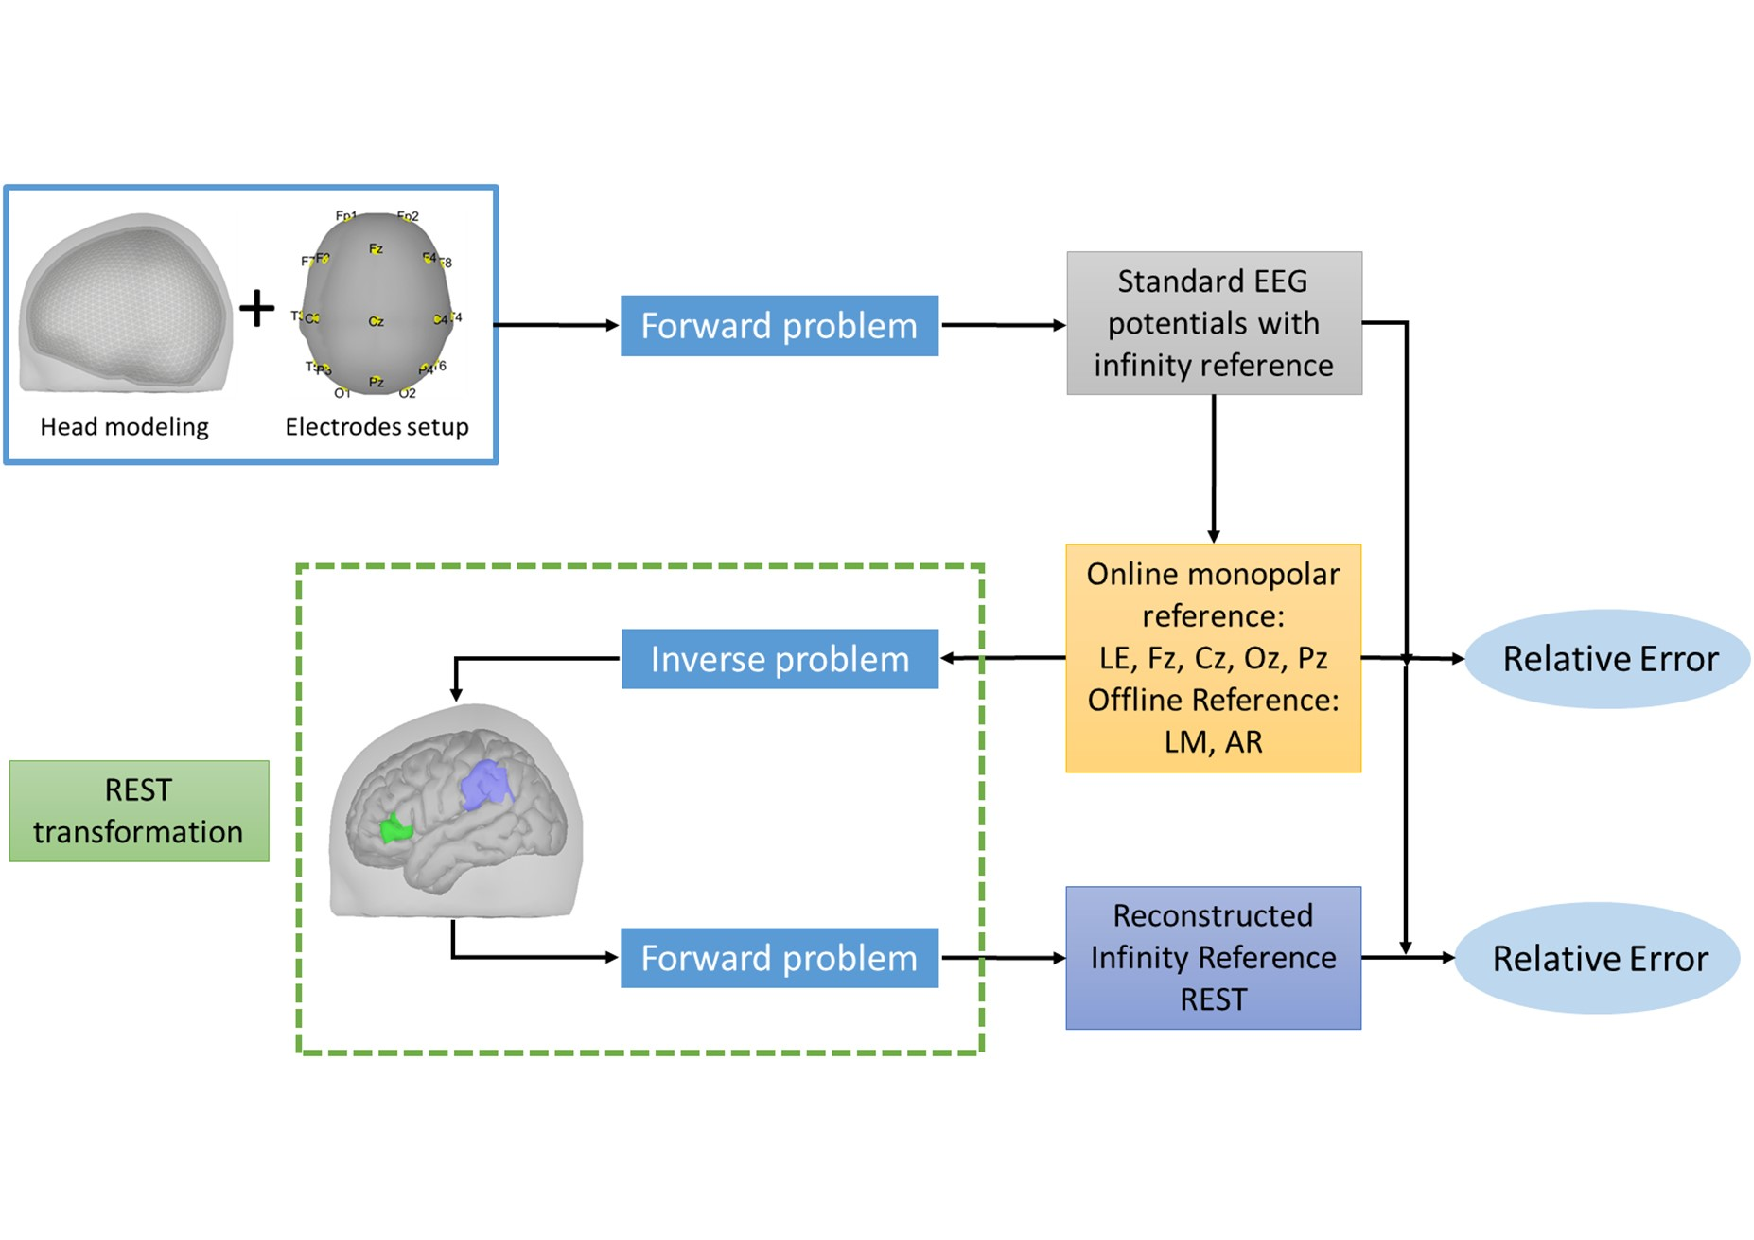
\includegraphics[width=0.6\textwidth,natwidth=610,natheight=642]{pic/2.1.pdf}
	\caption{标准脑电电位生成,参考转换,相对误差定义的流程图。给定头模型和电极配置,无穷远参考电位正演生成作为基标准, 标准电位再被转换为不同参考的其他记录。最后,转换参考下的电位与基准电位的相对误差关于参考模态、电极配置和一些其他因素交叉比较。}
	\label{2.1}
\end{figure}

\section{结果}

\section{本章小结}
本章中,我们全面研究了参考模态和电极配置如何影响脑电电势的准确性。我们发现无穷远参考和平均参考是两种有效的重参考方法,领先于单极参考或者连接耳参考。 从电极数量、头表区域、电极分布、偶极子源的位置与方向以及电极噪声和容积传导头模型角度进行比较研究,我们发现无穷远参考比平均参考更加鲁棒地矫正失真的电势,同时发现平均参考的的性能与电极数量并无关系但是受到电极分布覆盖基于偶极子源方向的影响。 因此在将来的脑电研究中,我们推荐广泛尝试无穷远参考,当使用平均参考时应注意是否电极具有宽泛的覆盖头表。